\label{section: 6}
As already seen in section \ref{section: 4}, the generator exploits several basic commands to build the graph database. 
Concerning the application, it triggers neo4j library routines to manage the database changes and to guarantee its consistency. 
In this section, we report the behaviour of the most relevant commands and explore their employment within the Python code. \\*
Below, there is the list of commands: \\*
\begin{itemize}[leftmargin=*]
    \item \textbf{Creation of COVID exposures command.} It is triggered whenever the government employee inserts a positive test. At first, it collects all people IDs. Then, it builds the relationships according to the IDs found.
    \begin{figure}[h]
        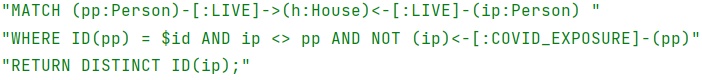
\includegraphics[width=\textwidth]{images/create_covid_exposure_command/family_contacts.png}
        \captionsetup{skip=7pt}
        \caption{\textit{Query that retrieves either flatmates' or relatives' IDs of a positive person.}}
    \end{figure}
    \begin{figure}[h]
        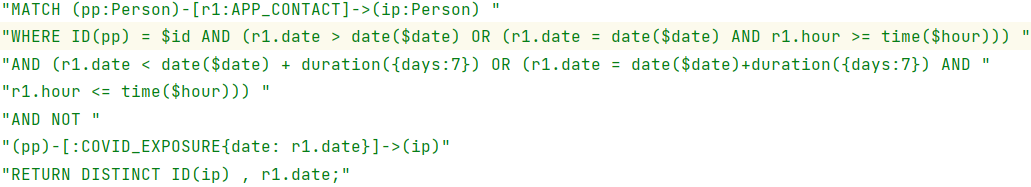
\includegraphics[width=\textwidth]{images/create_covid_exposure_command/app_contacts.png}
        \captionsetup{skip=7pt}
        \caption{\emph{Query that retrieves app contacts IDs for a positive person.}}
    \end{figure}
    \begin{figure}[ht]
        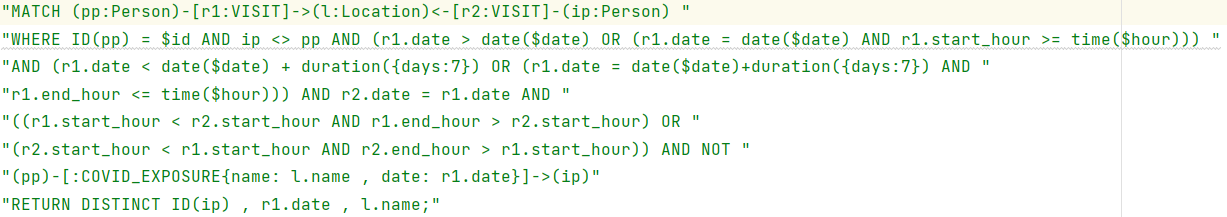
\includegraphics[width=\textwidth]{images/create_covid_exposure_command/visit_contacts.png}
        \captionsetup{skip=7pt}
        \caption{\textit{Query that retrieves people met by a positive person in a certain place.}}
    \end{figure}
    \begin{figure}[!htb]
        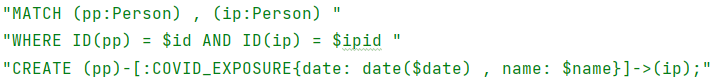
\includegraphics[width=\textwidth]{images/create_covid_exposure_command/exposed_people.png}
        \captionsetup{skip=7pt}
        \caption{\textit{Command run over all previously collected IDs to instantiate the exposures.}}
    \end{figure}
    \newpage
    \item \textbf{Deletion of possible exposures command.} It is triggered whenever the government employee inserts a negative test. It looks for the exposures that may have involved the negative tested person and, it deletes all of them.
    \begin{figure}[h]
        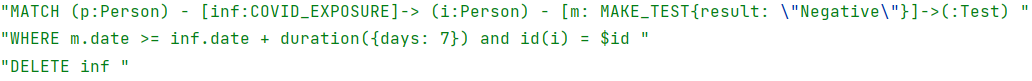
\includegraphics[width=\textwidth]{images/commands/delete_exposures.png}
        \captionsetup{skip=7pt}
        \caption{\textit{Deletion command. Note that the search is done by ID.}}
    \end{figure}
    
    \item \textbf{Update of personal information command}. Differently from the others above, this command is called when a generic user is modifying his information. It supports email and phone number changes.
    \begin{figure}[h]
        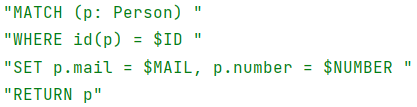
\includegraphics[scale = 0.75]{images/commands/info_update.png}
        \captionsetup{skip=7pt}
        \caption{\textit{Update of telephone number and email provided the person ID.}}
    \end{figure}
    
    \item \textbf{Creation of a new test command.} It adds the given \emph{date, hour and result} as attributes of the relationship.
    \begin{figure}[h]
        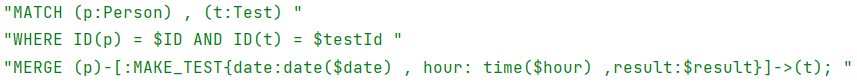
\includegraphics[width=\textwidth]{images/commands/add_new_test.png}
    \end{figure}
    \item \textbf{Creation of a new visit instance command.} It is activated whenever a location manager adds data related to a \emph{visit}. The \emph{date} is set by default to the current one, whereas the user has to specify the \emph{hour} as attribute of the relationship.
    \begin{figure}[!h]
        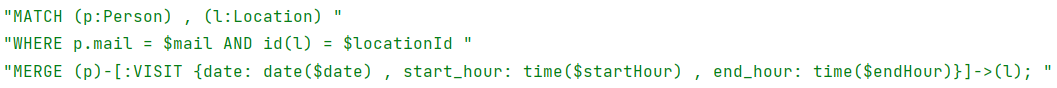
\includegraphics[width = \textwidth]{images/commands/visit_creation.png}
    \end{figure}
\end{itemize}
